% arara: xelatex: { shell: yes, synctex: yes }
% arara: biber
% arara: xelatex: { shell: yes, synctex: yes }
% arara: xelatex: { shell: yes, synctex: yes }
\RequirePackage[l2tabu, orthodox]{nag}
\documentclass[english,fira]{ist-report}

% -- Texto e codificação
\usepackage{anyfontsize}
\usepackage{pdflscape}



% -- Símbolos extra
\usepackage{amssymb}
\usepackage{textcomp}
\usepackage{gensymb}
\usepackage{cancel}

% -- Redefine margins
\geometry{top = 1cm}

% -- Bibliografia
\usepackage[
	backend = biber,
	style = alphabetic,
	sorting = ynt,
	%alldates=iso
	]{biblatex}
\usepackage{fvextra}
\usepackage{csquotes}

% --  Definições de imagens
\graphicspath{{graphics/}}
\usepackage{caption}
\usepackage{subcaption}
\usepackage{afterpage}
\usepackage{tabularx}

% -- Desenhar circuitos elétricos e lógicos
\usepackage{tikz}
\usepackage{pgfplots}
\usepackage{circuitikz}
\usetikzlibrary{arrows.meta,positioning,patterns,graphs}
\pgfplotsset{compat=1.15}
\pgfplotsset{table/search path = {data}}
\pgfplotsset{/pgf/number format/use comma,}

% -- Integrar código fonte
\usepackage{minted}
\usepackage{verbatim}
\usepackage{algorithm}
\usepackage{algpseudocode}

% -- Tabelas
\usepackage{booktabs}
\usepackage{makecell}

% -- Misc
\usepackage[disable]{todonotes}

% -- Funções matemáticas extra
\usepackage{siunitx}
\sisetup{
  math-ohm=\Omega,
  text-ohm=\ensuremath{\Omega},
}
\DeclareSIUnit{\lux}{LUX}


%\usepackage[sfdefault]{FiraSans}
%\renewcommand*\oldstylenums[1]{{\firaoldstyle #1}}
%\usepackage[mathrm = sym]{unicode-math}
%\setmathfont[
%    Path = ./fonts/,
%    Extension = .otf]{FiraMath-Regular}
%\usepackage{FiraMono}

\title{Distributed Real-Time Control Systems}

% TikZ and minted hotfix, cuz those are fun
\makeatletter
\global\let\tikz@ensure@dollar@catcode=\relax
\makeatother

\sisetup{math-micro=\text{µ},text-micro=µ}
\sisetup{math-ohm=\text{Ω},text-ohm=Ω}

%\definecolor{codebg}{rgb}{0.97,0.97,0.97}
%\setminted[c]{bgcolor = codebg, breaklines, linenos}
%\setmintedinline[c]{bgcolor = {}}

\setminted[c]{linenos, frame = leftline, breaklines}

\geometry{tmargin = 1.5cm}

\newrobustcmd*{\matr}[1]{\symbf{#1}}%{\mathbf{#1}}
\newrobustcmd*{\ccode}[1]{\mintinline{c}{#1}}

\newrobustcmd*{\ccheckmark}{\tikz\fill[scale=0.4](0,.35) -- (.25,0) -- (1,.7) -- (.25,.15) -- cycle;} 

\renewcommand{\mathbf}[1]{\symbf{#1}}

\renewcommand{\baselinestretch}{1.15}

\addbibresource{bibliography.bib}

\begin{document}

\begin{titlepage}

\begin{center}
	\vspace*{0.1\textheight}
	
\includegraphics[width = 0.4\linewidth, trim = {172.4pt 202.7pt 172.6pt 201.4pt}, clip]{IST_A_CMYK_POS}
	
	\vspace*{0.1\textheight}
	{\huge\bfseries Real-Time Cooperative Decentralized Control of a Smart Office Illumination System}
	
	\vspace*{0.03\textheight}
	{\Large Distributed Real-Time Control Systems Final Project}
	
	\vspace*{43.5mm}
	{\Large \begin{tabular}{l r} Daniel de Schiffart & \textbf{81479} \\ João Gonçalves & \textbf{81040} \\ Francisco Castro & \textbf{78655}\end{tabular}}
	
	\vspace{\fill}
	{\large Distributed Real-Time Control Systems}
	
	\vspace*{0.01\textheight}
	{\Large Master's Degree in Aerospace Engineering}
	
	\vspace*{0.01\textheight}
	{\large Instituto Superior Técnico}
	
	\vspace*{0.8cm}
	{\large\bfseries 2018/2019}
\end{center}

\end{titlepage}
\setcounter{page}{1}

\begin{abstract}
	In this technical report we will present the design and development of a LED-powered office illumination system that implements distributed real-time control to maintain comfortable levels of illuminance for its users. We will discuss the approaches done to the modelling of each sensor and corresponding LED and its individual control system, the method of communication between all connected sensor-LED pairs (henceforth referred to as desks), the interaction between the lights emitted by each desk and their joint effort to reduce lighting costs and maximize user comfort, and the gathering of relevant data for diagnostics.
	\newline
	
	\textit{\textbf{Keywords:}} Smart Office Illumination, Cooperative Distributed Control, Consensus Algorithm, Serial Communications, Arduino, Raspberry Pi, C++.
\end{abstract}

\setcounter{tocdepth}{2}
{\hypersetup{linkcolor = black} \tableofcontents}

\pagebreak
\section{Introduction}

In the last decade, the implementation of LED illumination systems has proven to be a low-energy consumption system in comparison to traditional approaches. As a consequence, this system is also low-cost, which has made possible to apply this kind of illumination devices on cars, offices and homes.

The adaptability of LED illumination systems has been used to improve energy optimization and comply with comfort levels. Distributed control systems have been presented as a possible solution for the problem, by keeping control of the occupation status of spaces and the illuminance values on them, taking into account external illumination levels.

In this project, a simple office-like scenario was considered. The considered approach to achieve the specifications stated above, rely on implementing luminance sensors (LDR) on each desk, as well as light emitting diodes (LED). Communication between each luminaire is also thought to be a key part on achieving a suitable real-time cooperative control system. Moreover, a distributed optimization algorithm (\textit{Consensus} algorithm) is also a key tool on the way to achieve the lowest possible energy consumption.

In this project, the simulation of such a scenario was achieved by considering each \textit{desk} to be composed by a LED, a LDR, a presence sensor (buttons) and communicational elements (Arduino). The entire office will be simulated by joining every \textit{desk} together inside a cardboard box. For simplicity reasons, two desks were considered throughout the project. Energy minimization will be achieved by controlling the dimming level of each LED, so that the illuminance levels on each desk are higher than a certain value (for an occupied \textit{desk}) or lower than another (unoccupied \textit{desk}). These values were defined in the development phase (section \ref{development}). 

Section \ref{sec:ind-controller} is devoted to the implementation of an independent control system for each \textit{desk}, whose goal is to set the illuminance level to a reference value, this value measured on its desk, with no cooperation.

In the second part (section \ref{sec:distr}), both desk cooperate, whose main goals are to ensure communication between themselves in order to achieve suitable illuminance optimization levels, and to allow the access of many different kinds of data by clients through a server, to be placed on a Raspberry PI module. 

In the remaining sections of the report, the results obtained with the cooperative distributed control system are presented and discussed.

\begin{figure}[ht]
    \centering
    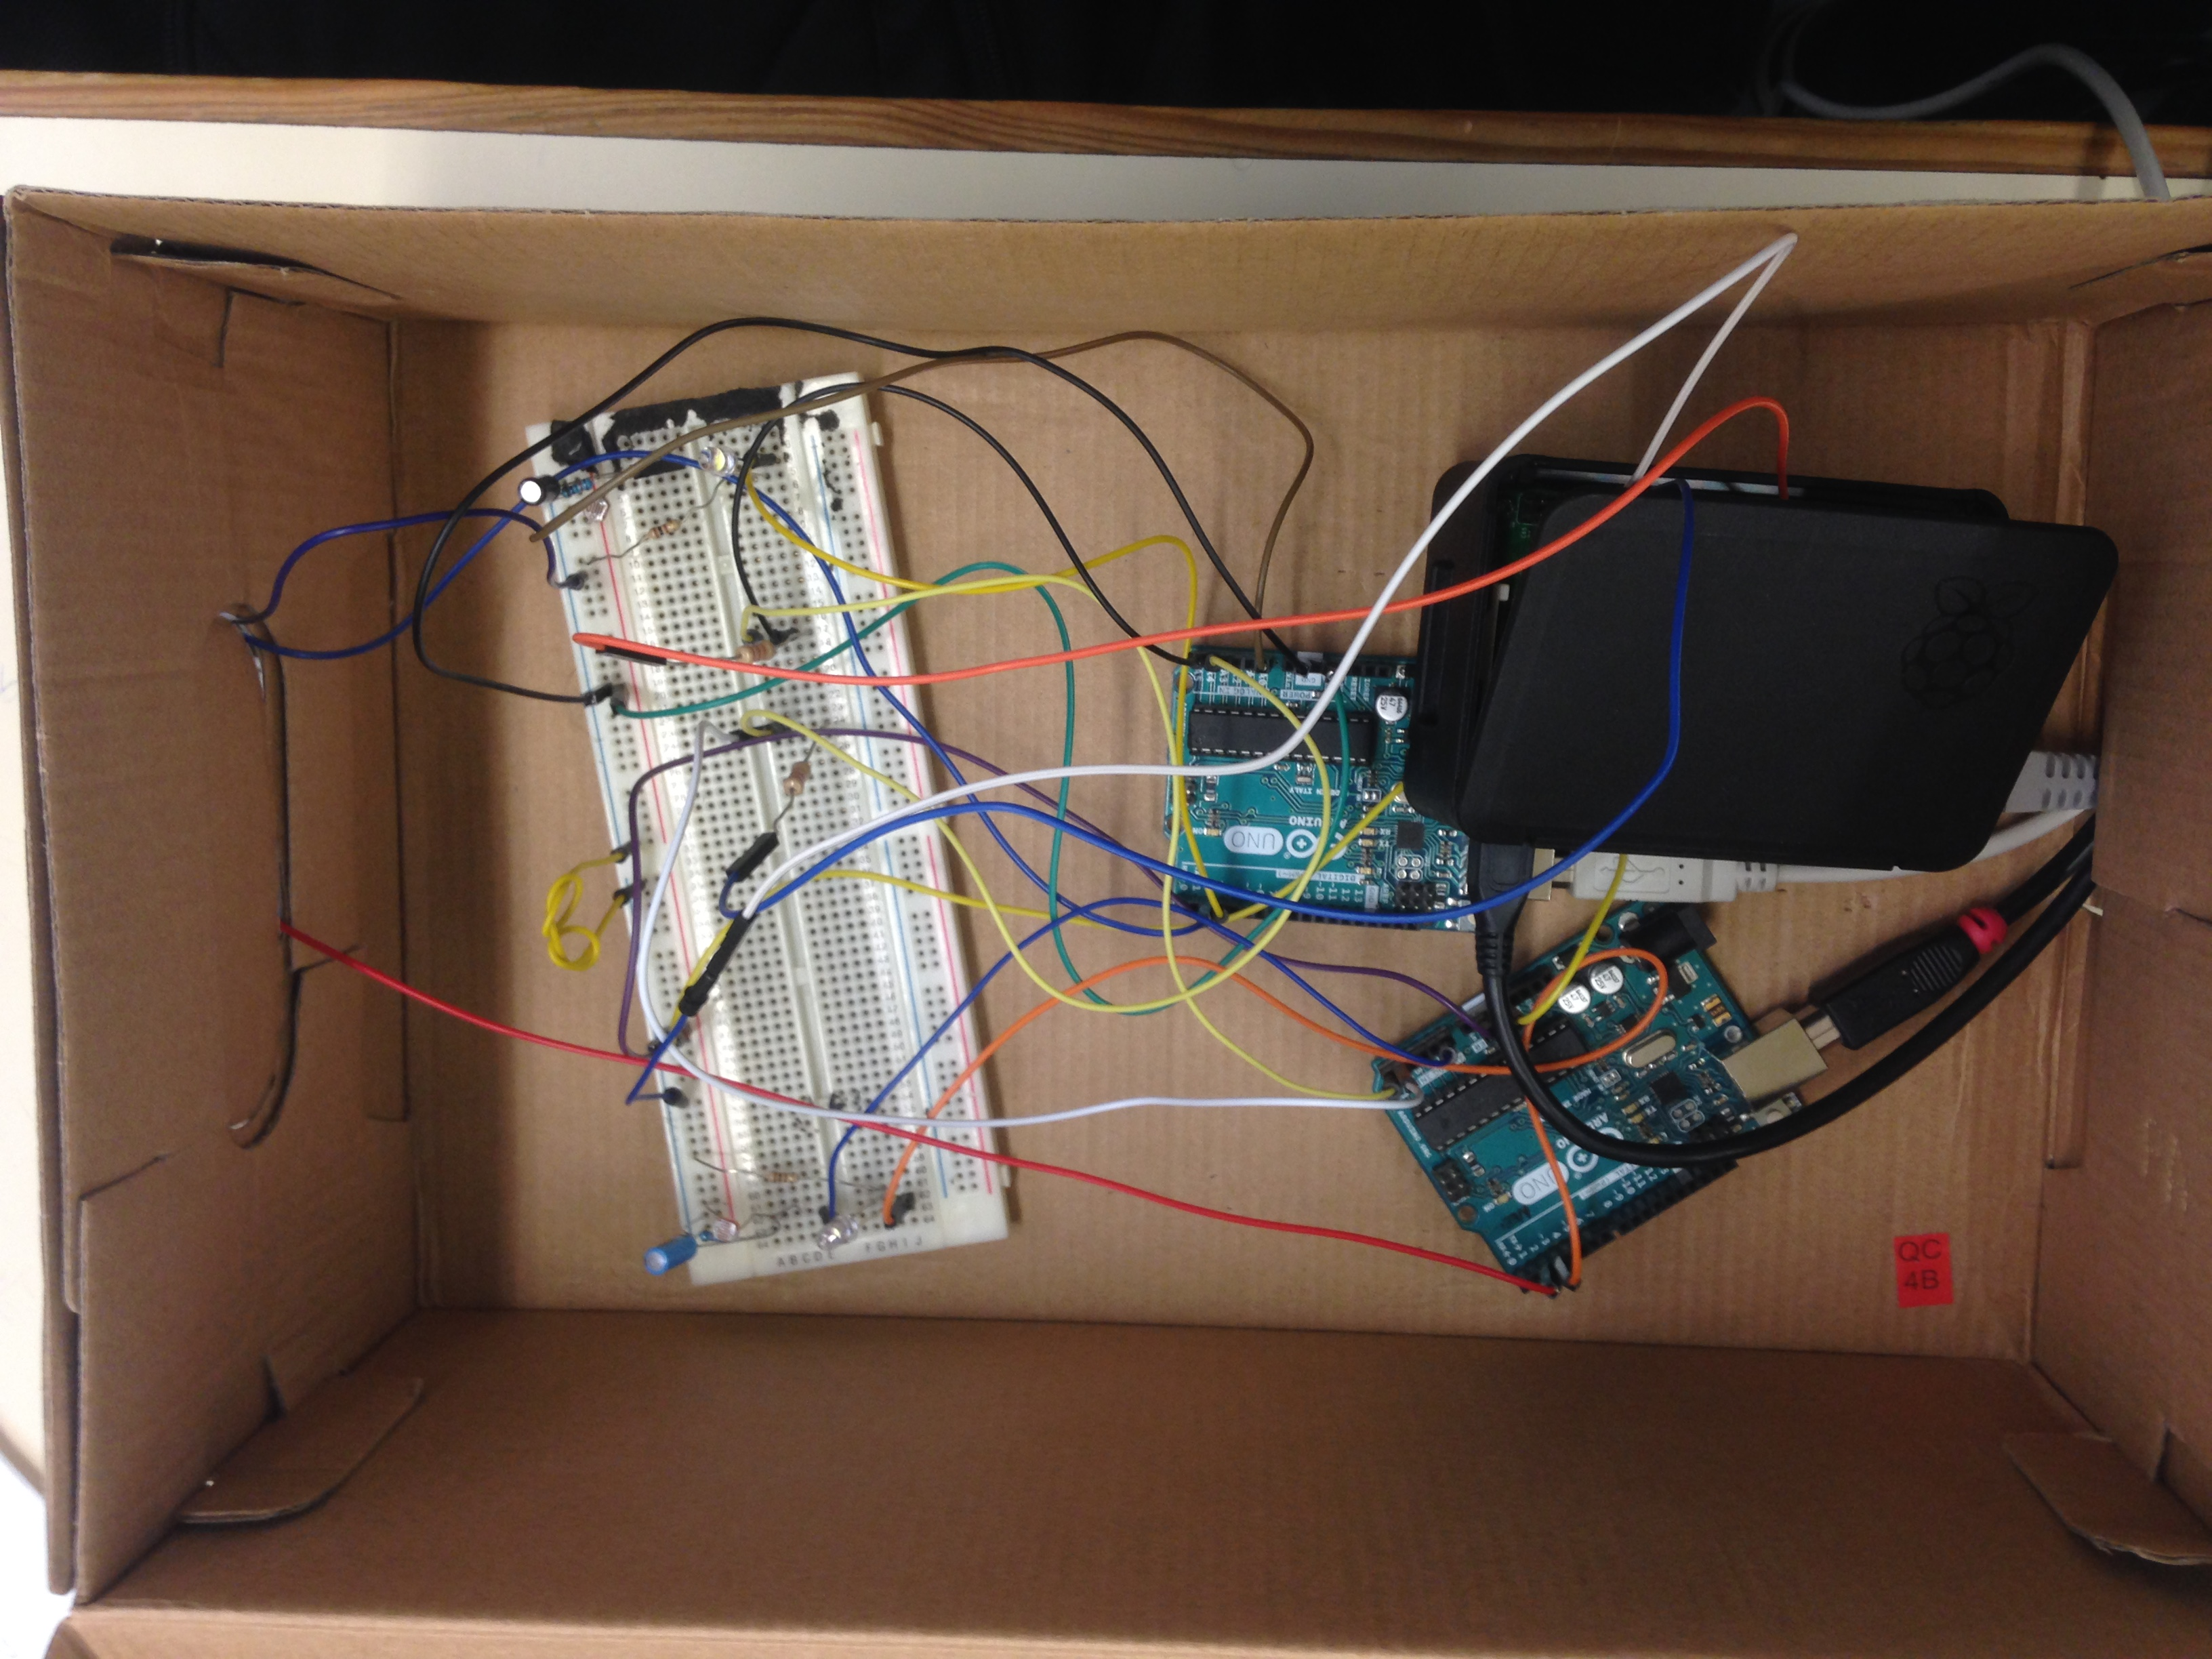
\includegraphics[height=8cm]{box.jpg}
    \caption{Hardware setup.}
    \label{fig:setup}
\end{figure}

\pagebreak
\section{Background and Concepts} \label{background_concepts}

In this section, some basic concepts introduced in classes which were useful for the project implementation are briefly described.

\subsection{Distributed Control}

A distributed decentralized coordinated control system, with explicit communication is used in on the project. This means there may be multiple controllers, where \textit{every controller makes a decision for it's own behaviour and the resulting system behaviour is the aggregate response} (decentralized). \textit{Each node communicates with the others} by explicit communication, \cite{slides}. 

A possible application of this solution is the Consensus algorithm, \cite{consensusbernardino}.

\subsection{Illuminance models}\label{sec:light}

The illuminance metric used to characterize the dimming level on each \textit{desk} is \si{\lux}. One \si{\lux} is equal to one \SI{1}{\lumen\per\meter\squared} (lumen per meter square). One \si{\lumen} characterizes the \textit{light produced by a light source emitting \SI{1}{\candela} (candela) over \SI{1}{\steradian} (steradian)}. Finally, a \si{\steradian} is the solid angle of a sphere section area, given by the division between the area of that surface and the sphere radius. A \si{\candela} is equal to \SI[quotient-mode=fraction]{1/683}{W} \textit{of green light per \si{\steradian} in a given direction}, \cite{slides}.

The luminous power incident on a surface is measured in \si{\lux}. The luminous flux of light emitted by a source is expressed in \si{\lumen}. The luminous intensity is expressed in \si{\candela}.

\subsection{Hardware concepts}

Each Arduino is responsible for processing and transmitting data at each node. The voltage for each LED is generated with a PWM (Pulse Width Modulation) signal. A PWM signal is a sequence of ones and zeros whose duration of each section is defined by a duty cycle (proportional to the analog voltage required). The value read by each LDR sensor is also received by the respective Arduino. Due to this, each Arduino also acts as a discrete microcontroller.

Discretization also adds quantization noise to the system. Moreover, the resolution (n-bit resolution) of a given quantization depends on the levels obtained with that process.

Serial communication between Arduinos (nodes) is ensured by the I2C communication protocol, where each Arduino may be a master or slave. \textit{A master can send data or request data from slaves, and a slave can read data or send data to the master}.

The Raspberry PI module will read from the I2C bus. This bus collects data from the inter-node communications.
\textit{The RPI will connect to the I2C bus in read-only mode and collects all messages transmitted in the bus for analysis. The RPI will also implement a server providing an interface for an application client. This application should be able to read the state of any luminaire and access system statistics.}

\section{Related Work}

This works focuses mainly on the achievement of a stationary state where low-energy consumption doesn't compromise comfort levels, by complying with the required illumination levels.

Similar projects also tried to achieve good levels of energy efficiency for luminaires with a centralized control system \cite{pandharipande2015centralized}. The brute-force algorithm is also another optimization approach as stated in \cite{mahoor2017hierarchical} for a street lighting system.

Inter-node communications and data handling are also very positive features of the system, because communication between nodes eliminates the need to define a central controller. During the simulation, it is also possible to access data, such as the current illuminance at a given \textit{desk} or the current occupancy state. 

\section{Development} \label{development}

\subsection{Illuminance measurement}

The luminaire node uses a light-dependant resistor (LDR) to measure illuminance, which is a non-linear component. 
Its resistance is approximately linear with illuminance in logarithmic units, and manufacturers provide a range of resistance for each illuminance value, as shown in figure \ref{fig:ldr-characteristic}.
The relationship between resistance, $R$, and illuminance, $L$, is given by:
\begin{align}
    \log_{10} R = m \log_{10} L + b, \label{eq:r-l-log}
\end{align}
with $m$ and $b$ being particular to each LDR, estimated with linear regression. See attached file \texttt{calibration.R}.

The resistance in turn is measured on a resistance divisor, as seen in figure \ref{fig:ldr-circuit}, and illuminance is computed as:
\begin{align}
\begin{aligned}
    R &= \frac{V_{cc} - v}{v/R_{aux}}\\
    L &= 10^{\frac{log_{10}R-b}{m}}, 
\end{aligned}
\label{eq:L-calc}
\end{align}
where $V_{cc}$ is \SI{5}{\volt}, $R_{aux}$ is \SI{10}{\kilo\ohm} and $v$ is the measured voltage, which is necessarily in the range $[0-5]\SI{}{\volt}$. The capacitor helps to mitigate noise in the circuit.

\begin{figure}[ht]
    \centering
    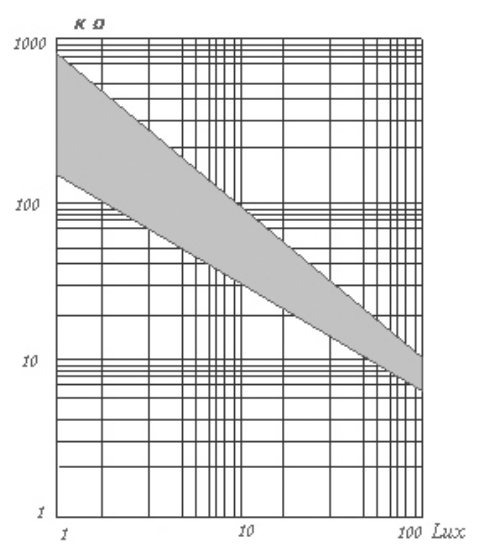
\includegraphics[height=5cm]{datasheet.png}
    \caption{LDR illuminance-resistance characteristic.}
    \label{fig:ldr-characteristic}
\end{figure}
\begin{figure}[ht]
    \centering
    \begin{tikzpicture}
    \node (start) at (0,0) [rground,rotate=180,label={0:\SI{5}{\volt}}] {};
    \path [draw] (start) to[vR,-*,label={$R$}] ++(0,-3) coordinate (center);
    \path [draw] (center) -- ++(-1.5,0) node (analog) [rectangle,draw,anchor=east] {Measure $v$ (\texttt{analogRead})};
    \path [draw] (center) to[R,l_={$R_{aux}$}] ++(0,-3) node [ground] {};
    \path [draw] (center) to ++(1.5,0) to[C,l={$C$}] ++(0,-3) node [ground] {};
\end{tikzpicture}
    \caption{LDR measuring circuit}
    \label{fig:ldr-circuit}
\end{figure}


\subsection{LED actuation}

The LED is driven by a digital pin with a pulse width modulation (PWM) signal, to emulate an analog output.
The frequency of the PWM signal is increased to \SI{980}{\hertz} to avoid the switching to be picked-up by the illuminance sensor, and cause unnecessary noise \cite{pwm-guide}.\footnote{This was not implemented at the time of the first demo.}

\subsection{Dynamical system modelling}

As discussed in section \ref{sec:light}, illuminance at any point changes instantly when a light source changes its radiated power.
However, in measured illuminance, there is a dynamic response, which is a property of the electric circuit that measures it. 
In particular, there is a delay, $\tau$, that should be estimated.

For a single luminaire node, there is a light source, the LED, and a sensor, the LDR, with a certain characteristic reflection path. The dynamic model of the measured illuminance to the LED power is assumed to be 1st order linear, as:
\begin{align}
    \frac{L(s)}{P(s)} = \frac{K_0(x)}{1+s\tau(x)},
\end{align}
where $L(s)$ and $P(s)$ are the Laplace transforms of the measured illuminance and LED power respectively. $K_0$ and $\tau$ are a gain and time constant, a function of $x$ to symbolize that they depend on the environment, through a specif reflection path setup.

To be noted that the model in equation \ref{eq:model} is BIBO-stable.

Experimentally, the LED is driven by step signals and the illuminance is measured, in order to estimate $\tau$ and $K_0$ for a common operation condition (box closed, see figure \ref{fig:steps}). The value of $K_0$ was used in earlier stages to drive the feed-forward controller, although a better methodology to estimate this gain for a multi-node configuration is described in section \ref{sec:calibration}. The value of $\tau$ is measured to be \SI{20}{\milli\second}, and will influence the choice of sampling time. It is also verified that $\tau \approx RC$ for this circuit. See attached file \texttt{model\_estimation.R}.

\begin{figure}[ht]
    \centering
    \begin{tikzpicture}
    	\begin{axis}
    	    [width = 0.7\linewidth,
    	    xlabel = {Time (\si{\micro\second})},
    	    ylabel = {Voltage (\si{\milli\volt})},
    	    grid = both,]
    		\addplot [red] table [col sep = comma, x index = 1, y index = 0, mark = none] {data4_simple.csv};
    		\addplot [blue, y filter/.code={\pgfmathparse{#1 * 15}\pgfmathresult}] table [col sep = comma, x index = 1, y index = 2, mark = none]{data4_simple.csv};
    	\end{axis}
    \end{tikzpicture}
    \caption{Measured illuminance (as voltage $v$) for step actuation in the LED, box closed.}
    \label{fig:steps}
\end{figure}


\subsection{Individual luminaire controller}\label{sec:ind-controller}

The purpose of the controller is to actuate on the system in order to have the illuminance $L$ to follow a reference value $L_{ref}$. In this section, $L$ represents the physical illuminance, i.e. the true value, while $\Tilde{L}$ represents measured illuminance. The control signal is the LED duty cycle, represented here as $u$.

The controller is implemented with a feedback component and a feed-forward component, described separately.

\subsubsection{Feed-forward control}

The feed-forward control aims to set a constant actuation by predicting the necessary value so that the output converges to the reference value. 
It has the advantage of not requiring sensors and being fast, and in this problem it is used to speed-up the response of the feedback-only controlled system. 
For usage, it requires that the system is open-loop stable, and also requires precise modelling, and its 
main disadvantage is that it cannot reject disturbances, or completely remove steady-state error.

With the available model in equation \ref{eq:model}, it is clear that a feed-forward controller can be used, by having simply:
\begin{align}
    C_{ff}(s) \equiv \frac{u(s)}{L_{ref}} = \frac{1}{K_0},
    \label{eq:ff}
\end{align}
so that the system response is:
\begin{align}
    \Tilde{L}(s) = \frac{L_{ref}}{1+s\tau}, 
    \label{eq:response-ff}
\end{align}
which settles to the steady-state value $L_{ref}$.

\subsubsection{Feedback control} 
\label{feedback control}

A feedback controller is required to eliminate steady-state error and reject disturbances. 
The usage, however, introduces delay and subjects the system to noise from the sensor. 
It is also important to verify that stability is maintained.

For this problem, the used controller is a proportional-integrative controller (PI). 

The proportional term penalizes error, $e$, the difference between the measured value and the reference, getting the actuation closer to the required value.

The integral term integrates the error in order to remove it in steady-state, however it must always be combined with proportional control as it slows the system and deteriorates stability.

A derivative term is skipped, as it is amplifies high-frequency noise, especially after dicretization.
Its purpose is to penalize oscillations and stabilize the response faster, but the plant is not prone to oscillations itself, and the feed-forward controller helps speed-up the response.

Additionally, the PI algorithm implemented is a \emph{velocity algorithm}, as described in \cite{bennett1994real}, since the actuation in equilibrium is not $0$ for this system. It consists in calculating the velocity of change in control, $\Dot{u}$ with a PID controller, in this case just PI, such as:
\begin{align}
    C_{fb}(s) \equiv \frac{U(s)}{E(s)} = \frac{1}{s}K_P\left( 1 + \frac{K_I}{s} \right),
    \label{eq:fb}
\end{align}
with $E(s) \equiv L_{des}(s)-\Tilde{L}(s)$, and $K_I$, $K_P$ gains to be chosen. $L_{des}$ is the "desired illuminance", covered next.

The choice of gains is done experimentally, based on the Ziegler Nichols frequency response method. 
In short, pure proportional gain is applied until the system starts to oscillate, which gives us the point on the Nyquist plot where the phase lag is $\pi$.
Then, the gains take some values based on the applied gain and observed frequency of oscillations.

As discussed in \cite{astrom2010feedback}, this method lacks robustness since too little information is used about the system. Therefore, the gains are manually tuned around the values given by this method. 
\begin{comment}
They are:
\begin{flalign*}
&K_P = 600& \\
&K_I = 0.00001&
\end{flalign*}
\end{comment}


\subsubsection{Feed-forward and feedback control}

The controllers are joined as shown in figure \ref{fig:ff+fb}. 
Normally, the feedback controller receives a reference value, like $L_{ref}$, however, with the usage of a feed-forward term, we already expect a certain response, and from the feedback controller it is only needed that the system loosely follows that first order response to the reference value.
Therefore, a \emph{predictor} is used to provide the feedback controller with a desired illuminance at each time, $L_{des}$. 

The value of $L_{des}$ can be predicted by converting equation \ref{eq:response-ff} to the time domain, considering that the reference value in this problem always varies in steps. 
Let $L_{ref}$ be the current reference and $L_{prev}$ the previous (constant) reference, and $t_0$ the instant when the reference changes. Then:
\begin{align}
    L_{des}(t) = L_{ref} - \left( L_{ref}-L_{prev} \right)\exp\left(-\frac{t-t_0}{RC}\right).
    \label{eq:predictor}
\end{align}
Obviously, $L_{des} \rightarrow L_{ref}$, as is expected in steady state.

\begin{figure}[ht]
    \centering
    \resizebox{\linewidth}{!}{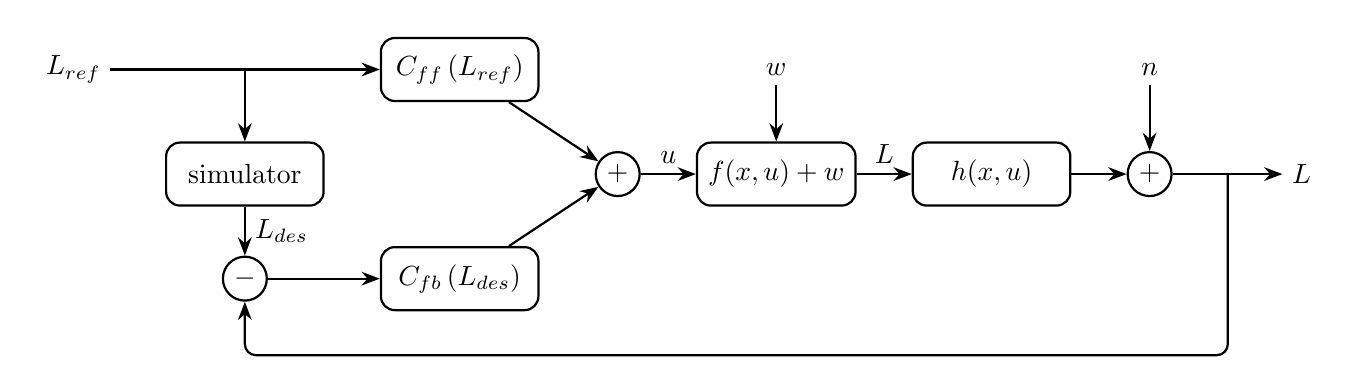
\begin{tikzpicture}[graphs/every graph/.style={edges={rounded corners,thick}}]
	\tikzstyle{block} = [rectangle,thick,rounded corners=5pt,draw,minimum height = 8mm, minimum width = 20mm,inner sep = 4pt];
	\tikzstyle{sum} = [circle,thick,draw,inner sep=2pt,align=center];
	\tikzstyle{skip loop} = [to path={-- ++(0,#1) -| (\tikztotarget)}]
	\matrix[row sep = 5mm, column sep = 7mm]{
		\node (xin) {$L_{ref}$}; & \coordinate (x1); & \node (controller1) [block] {$C_{ff}\left(L_{ref}\right)$}; & & \node (dist) {$w$}; & & \node (noise) {$n$}; & & \\
		& \node (ydes) [block] {simulator}; & & \node (sum1) [sum] {$+$}; & \node (system) [block] {$f(x,u) + w$}; & \node (sensor) [block] {$h(x,u)$}; & \node (sum2) [sum] {$+$}; & \coordinate (y_fb);	& \node (yout) {$\Tilde{L}$}; \\
		& \node (sumy) [sum] {$-$}; & \node (controller2) [block] {$C_{fb}\left(L_{des}\right)$}; & & & & & & \\
	};
	\graph [use existing nodes,edges=-{Stealth[]}]{
		xin -> controller1 -> sum1 -> [edge node={node[auto]{$u$}}] system -> [edge node={node[auto]{$L$}}] sensor -> sum2 -> yout;
		x1 -> ydes -> [edge node={node[auto]{$L_{des}$}}] sumy -> controller2 -> sum1;
		dist -> system;
		noise -> sum2;
		y_fb ->[skip loop = -23mm] sumy;
	};
\end{tikzpicture}}
    \caption{Feed-forward + feedback architecture. $w$ is disturbances, $n$ is sensor noise.}
    \label{fig:ff+fb}
\end{figure}

\subsubsection{Discretization}

The controller must be discretized in order to be implemented in the Arduino board. A fixed sampling time of $h=\SI{5}{\milli\second}$ is chosen, as it proved difficult to execute the calculations with smaller periods, although it should be noted that it is still large when compared with the characteristic time constant.

The integral controller is discretized using the Tustin transformation, which maps stable continuous-time poles to the inside of the unit circle in discrete-time, preserving stability. Additionally, it places a zero at $z=-1$ which attenuates noise, and suffers no delay. 
The result is:
\begin{align}
    i[k] = i[k-1] + \frac{h}{2}\left( e[k] + e[k-1] \right).
    \label{eq:integral-tustin}
\end{align}

The other integral which converts $\Dot{u}$ to $u$ is implemented with a backward  difference:
\begin{align}
    u[k] = u[k-1] + h\left( K_P (1+K_I i[k]) \right).
\end{align}

\subsubsection{Implementation}

For implementation in the luminairs, some additions are made:
\begin{enumerate}
    \item A 3-sample median filter is added to the sensor output, taking 3 measurements every control loop. This reduces sensor noise even further at a low computational cost.
    \item An error deadzone is added, to prevent flicker when the illuminance is still close to the reference value. The digital sensor readings only allows certain values of illuminance to be possible, so a small error is unavoidable. The deadzone behaves as:
    \begin{align}
        e = 
        \begin{cases}
            e-\epsilon, & \text{if } e>\epsilon \\
            0,          & \text{if } -\epsilon<e<\epsilon \\
            e+\epsilon  & \text{if } e<-\epsilon,
        \end{cases}
        \label{eq:deadzone}
    \end{align}
    where $\epsilon$ is set to a value in \SI{}{\lux} corresponding to the resolution interval of this signal.
    \item An anti-windup mechanism is added, by cancelling integration. This prevents windup when the actuator saturates, and greatly improves performance, for example when the box is opened and closed.
    \item Branching is kept to a minimum, and only important operations are done before the for the current actuation is set. In particular, writing to serial monitor and anti-windup are done after \texttt{analogWrite}. This minimizes the computation delay and also jitter. 
    \item Sampling time is measured with an interrupt on \texttt{Timer 1}, which raises a flag to enable control on the main problem loop. This allows for very precise scheduling of the control procedure, while not ignoring other possible interrupts.
\end{enumerate}

The final controller is present in annexed file \texttt{controller.h} as a class method. Algorithm \ref{al:controller} describes the controller. In this, $d$ is a \textit{reference dimming}, obtained from the distributed algorithm as described in section \ref{sec:distr}.

\begin{algorithm}[ht]
  \caption{PI + feed-forward control algorithm, called by an interrupt with period \SI{5}{\milli\second}.}
  \label{al:controller}
  \begin{algorithmic}[1]
    \Require $L_{ref}$, $d$
    \State $s \gets $\Call{median3}{\textit{3 measurements from sensor}}
	\State $L \gets $\Call{compute\_lux}{$s$}
	\State $ff \gets d$
	\State $L_{des} \gets $\Call{simulator}{}
	\State $e \gets $\Call{deadzone}{$L_{des}-L$}
	\State $i \gets i + \frac{h}{2}(e+e_{prev})$
	\State $u \gets u + h \cdot K_P (1+K_I i)$
	\State \Call{Write}{$u+ff$}  \Comment{Actuation}
	\If{$u+ff$ is saturated}     \Comment{Anti-windup}
	    \State $i \gets i - \frac{h}{2}(e+e_{prev})$
	    \State wrap $u+ff$ to the actuation bounds
	\EndIf
	\State $e_{prev} \gets e$
  \end{algorithmic}
\end{algorithm}

\subsection{Inter-node communications} \label{sec:comms}

Arduino nodes communicate via I2C bus. The communication protocol consists of a fixed message size, with a control byte for defining the contents of the data. From \texttt{comms.h}:
\label{lis:dataformats}
\begin{minted}[linenos, firstnumber = 19, frame = leftline]{c}
enum MsgCode : uint8_t{

    calibration_request,
    data,
    cont,
    acknowledge,
    consensus_data,
    consensus_stop,
    consensus_new,
    sampling_time_data,
    none,
};
\end{minted}
\begin{minted}[linenos, firstnumber = 35, frame = leftline]{c}
typedef struct msg{
    MsgCode code;    //!< Message code
    uint8_t address; //!< Sender's I2C address
    uint8_t aux1;    //!< field for data
    uint8_t aux2;    //!< field for data
    float value[3];  //!< field for data

}message_t;
\end{minted}
The message is fixed to 16 bytes which is the maximum size usable by the PigPio library on the Raspberry Pi.
All messages are sent as broadcasts, some are for logging purposes while others are used by the distributed control algorithm and calibration procedures. The purpose of the message is identified by its code, and the nodes are permanently listening for incoming messages. The code also identifies what variables are sent on the data fields.

Physically, the bus is a line between the Arduinos' SDA and SCL pins, which operates at logical levels \SI{0}{\volt} - \textit{LOW} and \SI{5}{\volt} - \textit{HIGH}. 
The Raspberry, however, has logical levels \SI{0}{\volt} - \textit{LOW} and \SI{3.3}{\volt} - \textit{HIGH}, therefore the connection is made with resistors to provide appropriate voltage drop, as shown in figure \ref{fig:i2c}.

\begin{figure}[ht]
	\centering
	\resizebox{0.5\linewidth}{!}{\begin{tikzpicture}
	\tikzstyle{arduino} = [draw,minimum height=80,inner sep=30];
	\tikzstyle{wire} = [];
	\node at (0,0) (ard1) [arduino] {\Large Arduino 1};
	\node (ard2) [right=4cm of ard1,arduino] {\Large Arduino 2};
	\node (rpi) [above=2cm of ard2,arduino] {\Large Raspberry Pi};
	\path (ard1.north east) to node (ard1_scl) [auto, swap, align=right] {\ttfamily SCL} ++(0,-3);
	\path (ard1.north east) to node (ard1_sda) [auto, swap, align=right] {\ttfamily SDA} ++(0,-4);
	\path (ard1.north east) to node (ard1_gnd) [auto, swap, align=right] {\ttfamily GND} ++(0,-5);
	\path (ard2.north west) to node (ard2_scl) [auto, align=left] {\ttfamily SCL} ++(0,-3);
	\path (ard2.north west) to node (ard2_sda) [auto, align=left] {\ttfamily SDA} ++(0,-4);
	\path (ard2.north west) to node (ard2_gnd) [auto, align=left] {\ttfamily GND} ++(0,-5);
	\path (rpi.north west) to node (rpi_19) [auto, align=left] {\ttfamily 19} ++(0,-3);
	\path (rpi.north west) to node (rpi_18) [auto, align=left] {\ttfamily 18} ++(0,-4);
	\path (rpi.north west) to node (rpi_gnd) [auto, align=left] {\ttfamily GND} ++(0,-5);
	\draw (ard1_scl) -- (ard2_scl) (ard1_sda) -- (ard2_sda) (ard1_gnd) -- (ard2_gnd);
	\path (ard1_scl) ++(1.7,0) coordinate (coord1);
	\path (ard1_sda) ++(2.4,0) coordinate (coord2);
	\path (ard1_gnd) ++(3.1,0) coordinate (coord3);
	\draw (coord1) to [short,*-,R] (coord1 |- rpi_19) to [short,-] (rpi_19.west);
	\draw (coord2) to [short,*-,R] (coord2 |- rpi_18) to [short,-] (rpi_18.west);
	\draw (coord3) to [short,*-] (coord3 |- rpi_gnd) to [short,-] (rpi_gnd.west);
\end{tikzpicture}
}
	\caption{Arduino and Raspberry Pi setup.}
	\label{fig:i2c}
\end{figure}

\subsection{Distributed control} \label{sec:distr}

The distributed control system was based on the Consensus Algorithm as stated in \cite{consensusbernardino}.

This optimization approach can be applied for $n$ nodes. However, in this project, only two nodes are used, with indexes given by $i=1, 2$. This distribution control system relies on two main parts: inter-node communication for exchange of information and optimization of a cost-function.

First of all, each node saves the local illuminance lower bound, $L_i$, the local external illuminance influence, $o_i$, the local cost coefficient, $c_i$, the local actuator bounds (to be $0$ and $100$ in this case), the coupling gains from the other luminaire to itself, $k_{ji}$ and a global optimization parameter, $\rho$.

Then, iterations start in order to optimize the current state of the system so that the sum of the cost functions (equation \ref{eq:cost_function}) from both nodes is on its lowest possible value.

\begin{align}
    f_i(\textbf{d}) = 
        \begin{cases}
             \textbf{c}_i^T \textbf{d}  & \text{if} {0 \leq d_i \leq 100 \enspace \text{and} \enspace \sum_{j=1}^{N} k_{ij}d_j \geq L_i - o_i} \\
             +\infty  & \text{otherwise}
       \end{cases} \quad
    \label{eq:cost_function}
\end{align}

with

\begin{align*}
    \textbf{d} & = [d_1 \enspace ... \enspace d_N]^T \\
    \textbf{c}_i & = [0 \enspace ... \enspace c_i \enspace ... \enspace 0]^T
\end{align*}

The consensus algorithm distributes the computation over the nodes. Each node holds a copy, $\textbf{d}_i$ of the global variable $\textbf{d}$ at every iteration.

The performed iterations focus on updating the dimming for each node and communicating them to every node. The average dimming of all nodes, $\textbf{d}_{av}$, and a local variable of Lagrange multipliers, $\textbf{y}_i$ are also updated, according to the equations stated in \cite{consensusbernardino}. 
At each iteration, a feasibility check of the obtained dimmings is also performed. The dimming to be taken at each iteration is given, at a first stage by the solution in the interior. If it is not feasible, the solutions in the border are evaluated and the minimum feasible solution is taken.

\subsubsection{Implementation details}

Implementation was made for a 2-node case only. For every restart, $\textbf{d}_i$, $\textbf{d}_{av}$ and $\textbf{y}$ are set to $\textbf{0}$. A node computes its proposal for $\textbf{d}$, then sends that via I2C with the message code \ccode{consensus_new}. When it is not the first iteration, the message code is \ccode{consensus_data}. 

After sending a copy of $\textbf{d}$, the node does not perform another iteration until it receives the peer's copy. With this, the message protocol is asynchronous, not request-response driven, but the alternation in messages is guaranteed for the algorithm to succeed. 

When the averaging of of $\textbf{d}$ does not change the previous values by more than \SI{0.5}{\percent}, the algorithm is said to have reached its solution, optimal by definition. Then, the iterations are stopped, with the message code \ccode{consensus_stop}.

Only after this happens are the references updated. While the consensus algorithm is being executed, the older references are still in place, and a new session of the consensus is started every time a lower bound is changed (the desk occupancy state changed).

On the Arduino code, the consensus is included within \mintinline{cpp}{Class Controller}, and the communication functions in the module \texttt{comms.h}.

The outputs of the consensus algorithm are dimmings, $\textbf{d}_{sol}$, but the controller accepts a reference in \SI{}{\lux}. This reference is used computing $\textbf{l}$ with equation \ref{eq:model}, discussed in the next section.
The value of $\textbf{d}_{sol}$ are still used as feed-forward gains.

The result given by this implementation was tested against that which was given by the Matlab script provided by the course staff, by hard-coding all conditions the as same.  

\subsection{Model calibration} \label{sec:calibration}

The illuminance at each \textit{desk} follows the model:
\begin{gather}
  L = K \matr{d} + \matr{o} \nonumber \\ 
  \left[\begin{array}{c} l_{1}\\ l_{2} \end{array}\right] =
  \left[\begin{array}{cc}
	k_{11} & k_{12}\\
	k_{21} & k_{22}
  \end{array}\right]
  \left[\begin{array}{c} d_{1}\\ d_{2}\end{array}\right]+
  \left[\begin{array}{c} o_{1}\\ o_{2} \end{array}\right]
  \label{eq:model}
\end{gather}
where $l_i$, $d_i$ and $o_i$ are the illuminance, LED power (in percentage) and background illuminance at desk $i$, respectively. The purpose of the calibration is to find the values for $k_{ij}$ and $o_i$ for a given office layout.

The calibration is performed by turning the luminairs synchronously and taking measurements. One node takes initiative and sends a message to trigger the process. First, both LEDs are switched off and $o_i$ is measured.
Then, node 2 turns on its LED, measures the resulting illuminance and computes $k_{22}$, and sends the illuminance to node 1. Receiving this value, node 1 can also measure its illuminance and compute $k_{21}$. The operation inverts and $k_{12}$ and $k_{11}$ are determined. In the end, nodes share the results.

\subsubsection{Implementation details}

The previous procedure is implemented as its own module, with a special communication protocol. The flow chart in figure \ref{fig:calib} illustrates messages sent and summarizes the finite-state machine.
Between changing the LED state and taking measurements, the nodes must sleep, to guarantee that the measurement is taken in steady state. For this, they were set to sleep for a length of time $10$ times the value of the system time constant, $\SI{10}{} \times \SI{20}{\milli \second} = \SI{0.2}{\second}$. 

It also should be noted that internally, the nodes are not distinguishable as 1 and 2. Each considers itself node 1 and the peer as 2, so the representation of the coupling matrix $K$ is transposed by both diagonals, and identically $o_1$ and $o_2$ are swapped.

\subsection{Data server}

The objective of the data server is to receive data from each desk and store it however it sees fit. It is also meant to provide this and other relevant data to other client programs that connect to it.

The data server was implemented in the provided Raspberry Pi computer and communicates with the Arduinos in much the same way as the Arduinos communicate among themselves, via I$2$C. Each Arduino sends a message to the implemented data server each sampling period with the relevant information about its current state, which the data server processes and stores accordingly.

\subsubsection{Arduino communication}

The data stored by the data server was balanced as to contain all the data that satisfies the project's client requirements but also to allow the message transmitted to be as short as possible. For reference, the client requirements for any desk $i$ can be found in table \ref{tab:client}.
\begin{table}[ht]
    \centering
    \begin{tabular}{l l}\toprule
        \textbf{Single-sample variables}        & \textbf{Cumulative variables (since last restart)} \\
        \midrule
        Illuminance                     & Time                          \\
        Duty cycle                      & Node energy spent             \\
        Occupancy state                 & Energy spent by all nodes     \\
        Lower bound                     & Node comfort error            \\
        Control reference               & Comfort error for all nodes   \\
        Background illuminance          & Node flicker                  \\
        Power consumption               & Node flicker for all nodes    \\
        Power consumption for all nodes &                               \\
        \bottomrule
    \end{tabular}
    \caption{Data requested by any connected clients.}
    \label{tab:client}
\end{table}

The server is meant to be able to retrieve this data at any moment from the Arduino and be able to provide it to the client upon request. It might be a bit too much to transmit from the Arduino to the Raspberry Pi server every sample; however, a lot of the data can be deduced from other values and, especially the cumulative variables, deduced from values stored in the server's own database.

We applied this reasoning by storing the initial value for each cumulative variable and adding to it for every received sample. By also adding the values for all desks stored and making the calculations for accumulation and the remaining variables within the server, we alleviated a lot of data load from the desk-server communication while still making sure all the request data is available to the client. We reduced the variables to be received by the server to the ones found in table \ref{tab:client_new}.
\begin{table}[ht]
    \centering
    \begin{tabular}{c}\toprule
        \textbf{Variable} \\
        \midrule
        Illuminance \\ Duty cycle \\ Occupancy state \\ Lower bound \\ Control reference \\ Instantaneous power consumption \\
        \bottomrule
    \end{tabular}
    \caption{Final variables transmitted by the Arduino to the server at each sampling time.}
    \label{tab:client_new}
\end{table}

As currently defined, each Arduino transmits messages using a format described in section \ref{sec:comms}. From that very section we can see \ccode{enum MsgCode} which describes the different types of messages transmitted, and only a select group of these formats can be accepted by the data server. The main format, \ccode{sampling_time_data}, contains the data included in table \ref{tab:client_new}, and is formatted according to table \ref{tab:ard2rpi_message}.

\begin{table}[ht]
	\centering
	\begin{tabular}[h]{l l c}\toprule
	    \textbf{Variable} & \textbf{Definition} & \textbf{Size (bytes)} \\
	    \midrule
	    \ccode{code}    & \ccode{sampling_time_data}    & $1$ \\
	    \ccode{address} & Arduino's I$2$C address       & $1$ \\
	    \ccode{aux1}    & Dimming value (resolution of \SI{1}{\percent})                & $1$ \\
	    \ccode{aux2}    & Lower bound value             & $1$ \\
	    \ccode{value[0]}& Illuminance value             & $4$ \\
	    \ccode{value[1]}& Power consumption             & $4$ \\
	    \ccode{value[2]}& Target illuminance value      & $4$ \\
	    \bottomrule
	\end{tabular}
	\caption{Formatting of the Arduino \ccode{sampling_time_data} message.}
	\label{tab:ard2rpi_message}
\end{table}

The background illuminances are the most notable missing feature when comparing tables \ref{tab:client_new} and \ref{tab:ard2rpi_message} with table \ref{tab:client}. This particular variable was left out of the message by considering it constant after each calibration procedure, and therefore does not need to be resent for every sample. Again referring to the code from page \pageref{lis:dataformats}, it makes use of the \texttt{data} message type transmitted by one of the Arduinos to set the value of the background illuminance for the program's runtime.

A final feature from the server's one-sided communication with the desk Arduinos is the auto-reset function, which detects a calibration procedure and resets the program. This resets the database and readies the program for the start of new time period of data acquisition. This detection is done using the \ccode{calibration_request} data format analogous to the ones used previously, which starts the reset procedure.

\subsubsection{Data storage}

The data received from the desk Arduinos is processed by the server upon reception and stored, divided in the program's data segment and heap. The stored data format can be seen in the \texttt{desk\_t} struct of the \texttt{data\_structures.hpp} file:
\begin{minted}[linenos, firstnumber = 4, frame = leftline]{cpp}
typedef struct desk{
    double illuminance; // Current illuminance in LUX
    double duty_cycle; // Current LED applied duty_cycle, from 0 to 1
    int occupancy; // ocupancy state, 0-empty 1-occupied
    double illuminance_lb; // Current illuminance lower bound
    double illuminance_bg; // Background measured at the last calibration
    double illuminance_ref; // Illuminance control reference
    double power; // Instantaneous power consumption
    uint32_t time_acc; // Timestamp of the last restart
    double energy_acc; // Accumulated energy
    double comfort_error_acc; // Accumulated comfort error
    double comfort_flicker_acc; // Accumulated flicker error
    
    uint32_t comf_err_samples; // Samples where there was confort error
    uint32_t samples;
    double l_prev; // Illuminance in the i-1 previous sample
    double l_pprev; // Illuminance in the i-2 previous sample
} desk_t;
\end{minted}
and in \texttt{main.cpp}:
\begin{minted}[linenos, firstnumber = 41, frame = leftline]{cpp}
const int desk_count = 2;
desk_t desks[desk_count]; //!< Data structure to store last sample desk info
std::pair< std::deque< std::pair<float, float > >,
        std::deque<std::pair<float, float> > > last_minute_buffer; 
        /*!< Deque to hold last-minute buffer of values for dimming and LUX */
\end{minted}

This data is stored in a desk array, where each entry represents a desk connected to the server.
There is a \texttt{deque}, which is internally a doubly-linked list, used as a FIFO queue, to hold data for one minute's worth of illuminance and dimming values.

\subsubsection{Client I/O}

To integrate client applications, an I/O (input/output) interface was developed for an expected client application format. This interface was also developed so that it could handle multiple clients at the same time.

The initial approach to developing this I/O interface was to begin by considering a single client, and further on in the development stage expand this functionality to an arbitrary $n$ number of clients. The method of communication used were TCP sockets, and all the client communication was done asynchronously. This means that we can send the request data at any time, which will correspond to the last received data for any desk. This approach allows the server to handle more client requests than its synchronous counterpart (as often mentioned in the C10k problem).
This aspect of the server data processing does require careful memory management to avoid sending data while it is being received from the Arduinos. This topic will be covered in section \ref{sec:memorysync}.

The server handles each client connection request by starting a new \texttt{Session} class instance, and using it to listen and reply to that specific client's requests. Each of these type of objects uses the \texttt{boost asio} resources to create threads and perform most of the synchronization between threads.

\subsubsection{Memory management}\label{sec:memorysync}

The consequence of making use of threads for the handling of multiple clients means the need for a clear definition of how each thread access the server's memory and the prevention of conflicts in this access (\textit{i.e.\@} a client requesting data as it is being received from one of the Arduinos).

This memory management was done using shared memory and \texttt{mutex} (mutual exclusion) objects to prevent the aforementioned conflicts. This allows each thread to lock the segment of memory that it is using and unlock it after it is done, allowing the next thread in line to access that very same information.

These implementations were mainly done to prevent any client handling thread from accessing any desk's data if it is being written by the server with newly received data from a desk's Arduino. As clients only read data from the server, their access to the data is relatively unrestricted as reading data poses little threat to the validity of the stored data.

\subsubsection{Server classes}\label{sec:classes}

The server program works using two classes: the \texttt{Server} class, which accepts client connections, and holds the references to the IO service, and the \texttt{Session} class, which is responsible for handling all of one client's requests.

\paragraph{\texttt{Server}}

The server class only stores the interface for the usage of the IO service provided by the boost library. It listens on a port for client connections and launches a handler. 

\paragraph{\texttt{Session}}

The Session class is responsible for serving clients. Each instance serves one and only one client. All the requests and responses are asynchronous, and the the object is destroyed automatically when connection is lost or closed.
For this purpose, this class inherits from \texttt{enable\_shared\_from\_this}, introduced in C++11, so that it can create shared pointers to itself and this way manage its lifetime.

One limitation is the inability to only handle one client request at a time (there is no queue of requests in case many are sent in a short time), which is an issue that could be improved.
Another aspect that is not ideal, is the usage of UNIX timestamps as timekeeping all throughout the program, which could be done in a more straightforward way with the chrono library.

\subsection{Data collection}

Data collection is done via the Pigpio library, running on the only explicitly created thread. Every time a sample is received, the mutex is locked, the data is written, and the mutex is unlocked again, allowing clients client handlers to access the data. Also here, a broadcast is done on a condition variable to wake up threads waiting for data used in streaming.

\section{Experiments}

In this section, experiments are designed to evaluate the performance of the system operating in different conditions.
The results are presented in section \ref{sec:results}.

\subsubsection*{Experiment 1 -- PWM analysis}

This experiment consists of holding a constant duty cycle on a LED and measuring the output for different PWM frequencies. The variance of the measured noise is computed.

\subsubsection*{Experiment 2 -- Benchmarking}

In this experiment, the \ccode{micros()} function is used to time critical sections of code -- computation delay, communication times and jitter are characterized.

\subsubsection*{Experiment 3 -- Local controller}

The performance of the controller is accessed in this experiment.
In particular, the step response of the system is measured, for the feedback only controller, the feed-forward only controller, and the joint controller. 
From the step response, the damping coefficient, rise time and overshoot are computed.

With the joint controller, the performance of the simulator is also measured, by comparing its output value with the actual measured illuminance.

\subsubsection*{Experiment 4 -- Anti-windup}

This is an experiment designed to test the closed-loop system in the presence of heavy disturbances, such that the actuation is likely to saturate.

The experiment starts by opening the box to intense external light, such that the background illuminance alone is higher than the reference value. 
This causes the computed actuation duty cycle to be lower than 0, but the illuminance doesn't decrease any further, which can cause the integral term to build up. 
The box is closed and the system must regain its original reference.

The experiment is repeated for the designed anti-windup scheme and for no anti-windup scheme implemented.

\subsubsection*{Experiment 5 -- Distributed controller}

On this experiment, some performance metrics are compared, for the the local and distributed controller modes. The most relevant one being total energy consumption, defined by:
\begin{align}
    E = \int \left( \sum_{i=1}^N \alpha c_i d_i \right)dt,
    \label{eq:energy}
\end{align}
where $c_i$ is the local cost for node $i$, and $\alpha$ is an arbitrary constant to convert $c_i d_i$ into units of power.
Note that $d \in [0-1]$, so the metric is non-negative.

The experiment consists of setting the local costs for node 1 to be $5\times$ that of node 2, and observing the illuminance at node 2 for some changes in the lower bound. 
The expected behaviour is for node 2 to increase its reference illuminance in order to \textit{help} node 1, minimizing global energy consumption.
On the same conditions, some metrics including global energy consumption are recorded, each after \SI{10}{\second} from a restart.

\section{Discussion and results} \label{sec:results}

\subsubsection*{Experiment 1}

The signals are shown in figure \ref{fig:pwm-results}. 

\begin{figure}[ht]
    \centering
    \begin{subfigure}[t]{0.47\linewidth}
        \centering
        \begin{tikzpicture}
            \begin{axis}
                    [width = \linewidth,
                    %xmin = 0, xmax = 1000,
                    %ymin = 0, ymax = 15,
                    xlabel = {Time ($\si{\micro\second}$)},
                    ylabel = {Illuminance ($\si{\lux}$)},
                    grid = both,
                    %legend pos = outer north east,
                    cycle list = {red,blue,cyan,teal,orange,purple,violet,brown,darkgray,magenta},]
                \addplot table [col sep = comma, x index = 0, y index = 1] {no_pwm_change.csv};
            \end{axis}
        \end{tikzpicture}
        %\missingfigure[]{Data from \texttt{no\_pwm\_changes.csv}}
        \caption{Signal for a PWM frequency of \SI{490}{\hertz} (the default.)}
        \label{fig:pwm-low}
    \end{subfigure}
    \hspace{\fill}
    \begin{subfigure}[t]{0.47\linewidth}
        \centering
        \begin{tikzpicture}
            \begin{axis}
                    [width = \linewidth,
                    %xmin = 0, xmax = 1000,
                    %ymin = 0, ymax = 15,
                    xlabel = {Time ($\si{\micro\second}$)},
                    ylabel = {Illuminance ($\si{\lux}$)},
                    grid = both,
                    %legend pos = outer north east,
                    cycle list = {red,blue,cyan,teal,orange,purple,violet,brown,darkgray,magenta},]
                \addplot table [col sep = comma, x index = 0, y index = 1] {with_pwm_changes.csv};
            \end{axis}
        \end{tikzpicture}
        %\missingfigure[]{Data from \texttt{with\_pwm\_changes.csv}}
        \caption{Signal for a PWM frequency of \SI{980}{\hertz} (the used value.)}
        \label{fig:pwm-high}
    \end{subfigure}
    \caption{Results for experiment 1.}
    \label{fig:pwm-results}
\end{figure}

The noise variance is \SI{0.4861}{\lux\squared} for the signal in \ref{fig:pwm-low}, and \SI{0.2952}{\lux\squared} for the signal in \ref{fig:pwm-high}. No improvements were made by further increasing the PWM frequency, and the noise appears identical to that of a natural light source.

\subsubsection*{Experiment 2}

The results are listed in table \ref{tab:benchmarking}.
With respect to jitter, the most important factors are the beginning of the control cycle and the computational time taken to compute a new actuation value.
The former is evidently very precise, the variance is residual, as it is signaled by an interrupt.
The computation time however is considerable, there is a delay between measurements are taken and actuation is ready. 
What is more important is for this delay to be approximately constant, so that the actuation is made in regular periods of time -- no jitter.
The evidence for that is the low variance of this delay, which was achieved by reducing branching.

Serial communications were only allowed for debugging purposes, so its effect is irrelevant. 
However, it is an accommodable cost for streaming a variable to the serial monitor, for example.

I2C communications are the biggest constraint to the node performance. 
Their speed is $100$\texttt{kbps}, which for 18 bytes (16 bytes with address and acknowledge) takes theoretically \SI{1.44}{\milli\second}, a value close to the measured one.
This has an important consequence -- as the sampling time is \SI{5}{\milli\second}, and for every consensus iteration each node has to exchange data, then only one iteration can be carried out per sampling time.

Another problem encountered that could not be solved was bus locking. 
Occasionally, the Arduino programs freeze on a call to \ccode{Wire.endTransmission()}, and only a restart on both devices resumes operation.

\begin{table}[ht]
    \centering
    \begin{tabular}{l|rr}\toprule
                                      & Mean                        & Variance                          \tabularnewline
\midrule
PI time until actuation               & \SI{1393}{\micro\second}    & \SI{39.16}{\micro\second\squared}     \tabularnewline
I2C Communication time ($16$ bytes)   & \SI{1761.79}{\micro\second} & \SI{694.3145}{\micro\second\squared} \tabularnewline
Serial communication time ($5$ bytes) &  \SI{384}{\micro\second}    & \SI{24}{\micro\second\squared}        \tabularnewline
Sampling time                         &  \SI{5.00}{\milli\second}   & \SI{0.3248}{\micro\second\squared}    \tabularnewline
\bottomrule
    \end{tabular}
    \caption{Results for measuring task time on the Arduino.}
    \label{tab:benchmarking}
\end{table}

\subsubsection*{Experiment 3}

Figure \ref{fig:controllers} shows the step response of different control schemes. 
From the time-series data of \ref{fig:contr-response}, some relevant parameters are calculated, and shown in table \ref{tab:controller-characteristics}.

The first conclusion is that the illuminance model is not entirely accurate, looking at figure \ref{fig:ffresponse}, the gain tracks well a reference of \SI{80}{\lux}, but not the \SI{150}{\lux} one.
However, it is fast, and does not overshoot.

The feedback controller tracks the reference with minimal error. 
It must be stated that the sensor reading is digital, and only $256$ different values are possible, therefore the resolution is not high enough to ensure a smaller steady-state error. 
Some overshoot is present, and the initial response is slow, evident by the rise time\footnote{Rise time is considered here to be the time taken for the signal to reach \SI{90}{\percent} of its final value.}.

Coupling the two controllers grants the best performance. 
Overshoot is eliminated by providing the feedback controller with the expected transient response, so that it does not overcompensate on actuation.

\begin{figure}[ht]
    \centering
    \begin{subfigure}[t]{0.47\linewidth}
        \centering
        \begin{tikzpicture}
            \begin{axis}
                    [width = \linewidth,
                    xmin = 0, xmax = 4,
                    ymin = 70, ymax = 160,
                    xlabel = {Time ($\si{\second}$)},
                    ylabel = {Illuminance ($\si{\lux}$)},
                    grid = both,
                    %legend pos = outer north east,
                    cycle list = {red,blue,cyan,teal,orange,purple,violet,brown,darkgray,magenta},]
                \addplot table [col sep = comma, x index = 0, y index = 1] {feedback.csv};
                \addplot coordinates {(-2,80) (6,80)};
                \addplot coordinates {(-2,150) (6,150)};
            \end{axis}
        \end{tikzpicture}
        %\missingfigure[]{Data from \texttt{feedback.csv}}
        \caption{Pure feedback controller.}
        \label{fig:fbresponse}
    \end{subfigure}
    \hspace{\fill}
    \begin{subfigure}[t]{0.47\linewidth}
        \centering
        \begin{tikzpicture}
            \begin{axis}
                    [width = \linewidth,
                    xmin = 0, xmax = 4,
                    ymin = 70, ymax = 160,
                    xlabel = {Time ($\si{\second}$)},
                    ylabel = {Illuminance ($\si{\lux}$)},
                    grid = both,
                    %legend pos = outer north east,
                    cycle list = {red,blue,cyan,teal,orange,purple,violet,brown,darkgray,magenta},]
                \addplot table [col sep = comma, x index = 0, y index = 1] {feedforward.csv};
                \addplot coordinates {(-2,80) (6,80)};
                \addplot coordinates {(-2,150) (6,150)};
            \end{axis}
        \end{tikzpicture}
        %\missingfigure[]{Data from \texttt{feedforward.csv}}
        \caption{Pure feed-forward controller.}
        \label{fig:ffresponse}
    \end{subfigure}
    \vskip\baselineskip
    \begin{subfigure}[b]{\linewidth}
        \centering
        \begin{tikzpicture}
            \begin{axis}
                    [width = \linewidth, height = 5cm,
                    xmin = 0, xmax = 5,
                    ymin = 70, ymax = 160,
                    xlabel = {Time ($\si{\second}$)},
                    ylabel = {Illuminance ($\si{\lux}$)},
                    grid = both,
                    %legend pos = outer north east,
                    cycle list = {red,blue,cyan,teal,orange,purple,violet,brown,darkgray,magenta},]
                \addplot table [col sep = comma, x index = 0, y index = 1] {feedforward_feedback.csv};
                \addplot coordinates {(-2,80) (6,80)};
                \addplot coordinates {(-2,150) (6,150)};
            \end{axis}
        \end{tikzpicture}
        %\missingfigure[]{Data from \texttt{feedforward\_feedback.csv}}
        \caption{Feed-forward + feedback controller.}
        \label{fig:contr-response}
    \end{subfigure}
    \caption{System output with successive step inputs of \SI{150}{} and \SI{80}{\lux}.}
    \label{fig:controllers}
\end{figure}

\begin{table}[ht]
    \centering
    \begin{tabular}{cccc}\toprule
         Overshoot & Damping, $\xi$ & Rise time & Settling time  \tabularnewline
        \midrule
         \SI{0.68}{\percent} & \SI{0.8499}{} & \SI{0.135}{\second} & \SI{0.191}{\second} \tabularnewline
        \bottomrule
    \end{tabular}
    \caption{Step response characteristics of the PI controller.}
    \label{tab:controller-characteristics}
\end{table}

\subsubsection*{Experiment 4}

The time plots for this experiment are present in figure \ref{fig:anti-windup}. 

In figure \ref{fig:windup}, when the box is closed, the illuminance drops close to $0$, and stays that way for close to a second, before regaining its reference of \SI{150}{\lux}. 
It is clear that when the external light was above the reference value, the error kept accumulating, so that after the bow was closed, the integrator must accumulate error in the inverse direction for a while, so that the actuation rises above $0$.

In figure \ref{fig:nowindup}, the illuminance still drops after the box is closed, but the actuation responds immediately, and the reference is regained faster.
This shows that cancelling integration is an adequate mechanism for preventing windup due to actuator saturation.

\begin{figure}[ht]
    \centering
    \begin{subfigure}[t]{0.47\linewidth}
        \centering
                \begin{tikzpicture}
            \begin{axis}
                    [width = \linewidth,
                    %xmin = 0, xmax = 1000,
                    %ymin = 0, ymax = 15,
                    xlabel = {Time ($\si{\second}$)},
                    ylabel = {Illuminance ($\si{\lux}$)},
                    grid = both,
                    %legend pos = outer north east,
                    cycle list = {red,blue,cyan,teal,orange,purple,violet,brown,darkgray,magenta},]
                \addplot table [col sep = comma, x index = 0, y index = 1] {windup.csv};
            \end{axis}
        \end{tikzpicture}
        %\missingfigure[]{Data from \texttt{windup.csv}}
        \caption{No anti-windup mechanism.}
        \label{fig:windup}
    \end{subfigure}
    \hspace{\fill}
    \begin{subfigure}[t]{0.47\linewidth}
        \centering
        \begin{tikzpicture}
            \begin{axis}
                    [width = \linewidth,
                    %xmin = 0, xmax = 1000,
                    %ymin = 0, ymax = 15,
                    xlabel = {Time ($\si{\second}$)},
                    ylabel = {Illuminance ($\si{\lux}$)},
                    grid = both,
                    %legend pos = outer north east,
                    cycle list = {red,blue,cyan,teal,orange,purple,violet,brown,darkgray,magenta},]
                \addplot table [col sep = comma, x index = 0, y index = 1] {antiwindup.csv};
            \end{axis}
        \end{tikzpicture}
        %\missingfigure[]{Data from \texttt{antiwindup.csv}}
        \caption{Anti-windup prevention by cancelling integration.}
        \label{fig:nowindup}
    \end{subfigure}
    \caption{Anti-windup performance.}
    \label{fig:anti-windup}
\end{figure}

\subsubsection*{Experiment 5}

The result for this experiment is presented in figure \ref{fig:comparison-distr} and table \ref{tab:metrics}. The lower bound for this experiment is defined as \SI{120}{\lux} for an empty desk, and \SI{250}{\lux} for an occupied desk. 

As expected, for an independent control architecture, the node only tries to minimize its local power usage, therefore it is obvious that the reference values are simply the lower bounds, as evidenced by figure \ref{fig:comp-independant}. On a side note, the same is also the case if both nodes have the same cost coefficients.

For the cooperative control architecture, it is clear from figure \ref{fig:comp-cooperative} that the illuminance value is considerably above the lower bounds. This is the optimal result found by the distributed control algorithm, because increasing the dimming on this node, where power is \textit{cheap}, and decreasing it on the other node, where power is \textit{expensive}, results in overall lower energy consumption.
It is also seen in this picture that the excess illuminance is higher while the desk is empty than while it is occupied, which is evidence that the solution is on the upper boundary for this node's dimming, for the occupied desk state. In other words, if it could increase its dimming more, it would. 

Some performance metrics are gathered in table \ref{tab:metrics}. It should be admitted though that it was challenging to take accurate measurements for the same conditions, and the data can be inaccurate. As expected, total energy spent is lower for the cooperative control type. Only slightly, because the test was carried out with both desks occupied, where the solution is maximum dimming on the node with lower cost. The same is true for power. Total comfort error is also lower because the reference value is higher than the lower bound for one of the nodes, so noise never causes the illuminance to go below the lower bound. As for flicker, there is no apparent reason for it to be higher or lower on any case, and the difference seen is most likely due to inaccurate measurements.

\begin{figure}[ht]
    \centering
    \begin{subfigure}[t]{0.47\linewidth}
        \centering
        % Tempo está em millisegundos.
        % Pinta uma linha horizontal em 120 e outra em 250
        %\missingfigure[]{Data from \texttt{stream2.csv}}
        \begin{tikzpicture}
            \begin{axis}
                    [width = \linewidth,
                    xmin = 114613, xmax = 116294,
                    ymin = 100, ymax = 290,
                    xlabel = {Time ($\si{\milli\second}$)},
                    ylabel = {Illuminance ($\si{\lux}$)},
                    grid = both,
                    %legend pos = outer north east,
                    cycle list = {red,blue,cyan,teal,orange,purple,violet,brown,darkgray,magenta},]
                \addplot table [col sep = comma, x index = 0, y index = 1] {stream2.csv};
                \addplot coordinates {(114000,120) (117000,120)};
                \addplot coordinates {(114000,250) (117000,250)};
            \end{axis}
        \end{tikzpicture}
        \caption{Node 2 illuminance, distributed control.}
        \label{fig:comp-cooperative}
    \end{subfigure}
    \hspace{\fill}
    \begin{subfigure}[t]{0.47\linewidth}
        \centering
        % Tempo está em millisegundos.
        % Pinta uma linha horizontal em 120 e outra em 250
        %\missingfigure[]{Data from \texttt{stream2\_ind.csv}}
        \begin{tikzpicture}
            \begin{axis}
                    [width = \linewidth,
                    xmin = 44067, xmax = 45589,
                    ymin = 100, ymax = 290,
                    xlabel = {Time ($\si{\milli\second}$)},
                    ylabel = {Illuminance ($\si{\lux}$)},
                    grid = both,
                    %legend pos = outer north east,
                    cycle list = {red,blue,cyan,teal,orange,purple,violet,brown,darkgray,magenta},]
                \addplot table [col sep = comma, x index = 0, y index = 1] {stream2_ind.csv};
                \addplot coordinates {(44000,120) (46000,120)};
                \addplot coordinates {(44000,250) (46000,250)};
            \end{axis}
        \end{tikzpicture}
        \caption{Node 2 illuminance, independent control.}
        \label{fig:comp-independant}
    \end{subfigure}
    \caption{Time responses for experiment 5, lower bound is switched from \SI{120}{\lux} to \SI{250}{\lux}.}
    \label{fig:comparison-distr}
\end{figure}

\begin{table}[ht]
    \centering
    \begin{tabular}{l|r|r}
        Metric & Independant control & Cooperative control \\
        \hline
        Total accumulated energy -- \texttt{g e T}              & \SI{8523.97}{\joule} & \SI{8490.16}{\joule} \\
        Total instantaneous power consumption -- \texttt{g p T} & \SI{864.45}{\watt}   & \SI{851.65}{\watt}  \\
        Total confort error -- \texttt{g c T}                   & \SI{4.5378}{\lux}  & \SI{2.6512}{\lux}  \\
        Total flicker error -- \texttt{g v T}                   & \SI{181.848}{\lux\per\second} & \SI{138.587}{\lux\per\second}
    \end{tabular}
    \caption{Performance metrics, taken \SI{10}{\second} after a restart.}
    \label{tab:metrics}
\end{table}

\section{Conclusion}

% Controlo centralizado vs não-centralizado

In the project, other distributed control approaches could be used, such as the centralized control architecture. The global results obtained with the non-centralized approach are satisfactory, but one doesn't know if other techniques could provide better outcomes. 

In \cite{pandharipande2015centralized}, a similar application with a central controller is implemented, which receives all the illuminance and occupancy information, and outputs the next dimming values of the luminaires. The results obtained with this approach have proven to be valid solutions, as they have shown negligible overshoot, some illuminance deviations and low energy savings. It also seems to comply with comfort requirements. In general, this approach seems to be as valid as the decentralized approach.

Despite that, non-centralized control has considerable advantages. It is less dependant on a single agent in order to work correctly, and thus is more fault-tolerant. Additionally, the computational overhead is evenly split among the available hardware, usually resulting in better performance. For the case of the consensus algorithm, each node only needs to search on its boundaries, yet the algorithm still guarantees optimality. With an increase in the number of nodes, the boundary regions grow exponentially if they are all considered at the same time in one centralized controller. We then conclude that distributed control has a huge potential on large networks of agents.

%feedforward vs sem feedforward

A PID controller with no feed-forward may also be a possible solution to implement. From its definition, a feed-forward segment allows a control system to act in terms of the inputs and not from the responses obtained. Thus, it is the major reason why little to none overshoot is seen on the results. However, it could be even smaller if the performed calibration was more exact. A control design with no feed-forward could be implemented, but the settling time would be higher.

On the server front, an effort was made to include modern conventions and programming paradigms. The boost library is extensive and allows the construction reliable IO agents for usage in real time control, as it maintains the low level requirements for computer control. 

\nocite{consensusbernardino}
\printbibliography[heading = bibnumbered]

\begin{table}[H]
    \centering
    \begin{tabular}{l|c|c|c}
        \toprule
        \textbf{Task}                                     & \textbf{Daniel} & \textbf{João} & \textbf{Francisco} \\
        \midrule
        Modelling and LDR calibration            &        &   R  &      I,R  \\
        \hline
        PID control                              &        &  I,R &      I    \\
        \hline
        Distributed control                      &        &   I  &      I,R  \\
        \hline
        Calibration                              &  I,R   &      &      I,R  \\
        \hline
        I2C Communications                       &  I,R   &      &           \\
        \hline
        Server: client services                  &  R     &   I  &           \\
        \hline
        Server: data management and concurrency  &  R     &   I  &           \\
        \hline
        Microcontroller programming              &  I     &   I  &           \\
        \hline
        C++ programming                          &        & I,R  &           \\
        \bottomrule
    \end{tabular}
    \caption{Member tasks completed. R-reporting, I-implementation.}
    \label{tab:my_label}
\end{table}

\pagebreak
\appendix

\section{Auxiliary schematics}
\begin{figure}[ht]
	\centering
	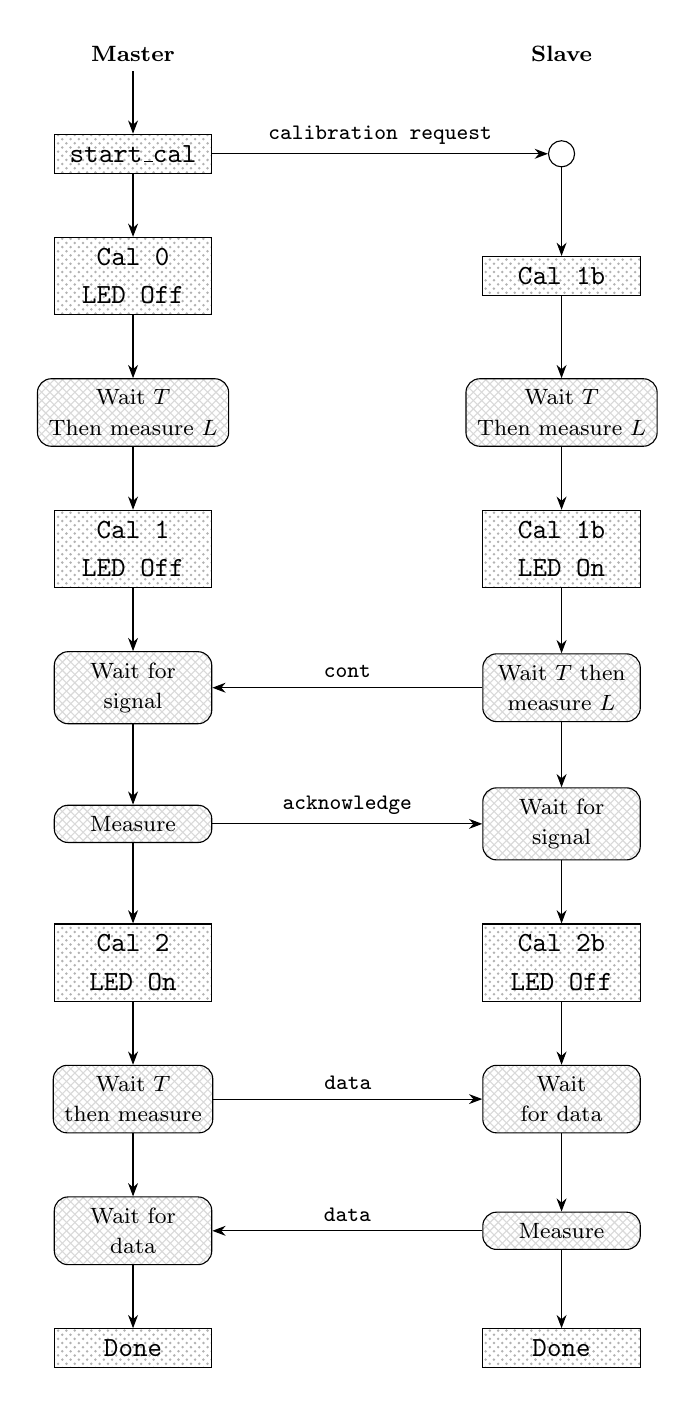
\begin{tikzpicture}
	\tikzstyle{every node}=[font=\footnotesize];
	\tikzstyle{stt}=[draw,rectangle,align=center,inner sep=4pt,minimum width=20mm,fill,pattern=crosshatch dots,pattern color=black!30!white,font=\ttfamily];
	\tikzstyle{stp}=[draw,rectangle,align=center,inner sep=4pt,minimum width=20mm,rounded corners=5pt,fill,pattern=crosshatch,pattern color=black!15!white];
	\tikzstyle{pth}=[draw,->,thick];
	\matrix[row sep=8mm,column sep=3cm]{
		\node (master_start) [] {\textbf{Master}};			& \node (slave_start) [] {\textbf{Slave}};			\\
		\node (m1) [stt] {start\_cal};						& \node (s1) [circle, draw] {};						\\
		\node (m2) [stt] {Cal 0 \\ LED Off};				& \node (s2) [stt] {Cal 1b};						\\
		\node (m3) [stp] {Wait $T$ \\ Then measure $L$};	& \node (s3) [stp] {Wait $T$ \\ Then measure $L$};	\\
		\node (m4) [stt] {Cal 1 \\ LED Off};				& \node (s4) [stt] {Cal 1b \\ LED On};				\\
		\node (m5) [stp] {Wait for \\ signal};				& \node (s5) [stp] {Wait $T$ then \\ measure $L$};	\\
		\node (m6) [stp] {Measure};							& \node (s6) [stp] {Wait for \\ signal};			\\
		\node (m7) [stt] {Cal 2 \\ LED On};					& \node (s7) [stt] {Cal 2b \\ LED Off};				\\
		\node (m8) [stp] {Wait $T$ \\ then measure};		& \node (s8) [stp] {Wait \\ for data};				\\
		\node (m9) [stp] {Wait for \\ data};				& \node (s9) [stp] {Measure};						\\
		\node (master_end) [stt] {Done};					& \node (slave_end) [stt] {Done};					\\
	};
	\graph [use existing nodes,edges=-{Stealth[]}]{
		master_start -> m1 -> m2 -> m3 -> m4 -> m5 -> m6 -> m7 -> m8 -> m9 -> master_end;
		s1 -> s2 -> s3 -> s4 -> s5 -> s6 -> s7 -> s8 -> s9 -> slave_end;
		m1 -> [edge node={node[font=\footnotesize\ttfamily,auto]{calibration request}}] s1;
		s5 -> [edge node={node[font=\footnotesize\ttfamily,auto,swap]{cont}}] m5;
		m6 -> [edge node={node[font=\footnotesize\ttfamily,auto]{acknowledge}}] s6;
		m8 -> [edge node={node[font=\footnotesize\ttfamily,auto]{data}}] s8;
		s9 -> [edge node={node[font=\footnotesize\ttfamily,auto,swap]{data}}] m9;
	};
\end{tikzpicture}

	\caption{Calibration procedure.}
	\label{fig:calib}
\end{figure}

\listoftodos

\begin{comment}
\pagebreak

\section{Report Structure}

This should be the report structure according to the class slides (Distributed Real-Time Control Systems, module 32).
\begin{description}
	\item[Abstract] A summary in less than 200 words;
	\item[Introduction] Motivation, challenges, main idea, objectives, outline;
	\item[Background/Concepts] Common knowledge required;
	\item[Related Work] State-of-the-art;
	\item[Development] Your approach, methodologies, innovations;
	\item[Experiments] Carefully explain the design of the experiments;
	\item[Results] Illustrate and comment on the results of experiments;
	\item[Discussion] Maybe in results;
	\item[Conclusions and Future] Critically comment on what was achieved and indicate points of improvement;
	\item[Bibliography]
	\item[Appendices]
\end{description}

Report should be less than 20 pages total, including everything.

\subsection{Discussable Topics}

\begin{itemize}
	\item Theoretical introduction and discussion of topic (office space illumination)
	\item Objective
	\item Composition of desks
	\item Illuminance measurement system
	\item LED actuation system
	\item Desk illumination model
	\item Desk illumination controller
	\item Gathering data
	\item Inter-desk communication
	\item Bus monitoring
	\item Calibration
	\item Distributed control algorithm
	\item Data server
	\begin{itemize}
		\item Performance metrics
		\item C++ implementation
	\end{itemize}
\end{itemize}

Implementation notes from stage 1.
\begin{itemize}
	\item Make plots for the different signals in the control system (references, control values, measurements) and compute metrics that show the correct operation of the system.
	\item Choose messages with short size and a high baud rate. Compute communication delays and verify that the communication time can be acommodated within the available control loop period.
	\item Graphically visualize the data in MATLAB or Excel.
\end{itemize}

Documentation notes from stage 1.
\begin{itemize}
	\item Take pictures of the interior and of the exterior of the box enclosing the luminaires. Make sure that you illustrate the position of the LED, the LDR and the emission/reflection path.
	\item Show plots of the steady state characteristic of the system. Show step responses of the system in different illuminance conditions.
	\item Characterize the jitter in your control system. How much does the sampling rate deviate from the desired one?
	\item Characterize the error in your feedforward controller. In particular, implement a predictor of your system and compute the average mean squared error between the prediction and the measurements.
	\item Characterize the dynamic characteristics of the feedback controller, in different illuminance conditions (overshoot, damping factor).
	\item Illustrate any improvements that you make to the basic feedback controller (feedforward term, anti-windup, etc) with plots of the time responses.
	\item Comment the Arduino code for your controller.
	\item Characterize the processing time taken by the control computation, serial communications and other computations.
\end{itemize}

Documentation notes from stage 2. \\
\textit{``In your report, please do not forget to address the following issues''}
\begin{description}
	\item[I$2$C communications] Indicate the average time required to send a request message and receive an answer.
	\item[C++ classes, sockets, parallelism] Indicate the C++ classes that are most relevant for coding the server running on the PC interfacing to the Arduinos.
	\item[Sockets] List the number of sockets used to implement the server. Describe the functions of the sockets.
	\item[Concurrency] Indicate the methodologies used in the server to implement parallelism in order to process requests from multiple clients.
	\item[Distributed control] Describe the implementation of the cooperative distributed controller.
	\item[Experiments] Perform experiments to compare results between the cooperative distributed contrller and the non-cooperative controller (independent local controllers). Plot the time response of both controllers in similar situations and create a table with their performance metrics.
\end{description}

\paragraph{Importante} Antes de desligar o Raspberry Pi, correr \texttt{sudo shutdown -h now} para evitar corrupção do sistema operativo.

\section{Illumination system calibration}

\subsection{Principles of the calibration procedure}

\section{Optimização do Sistema Distribuído}

\begin{gather*}
	u^* = \text{argmin}\,J(x, \mu) \\
	l_i = \sum^n_{j=1} d_j k_{ij} + o_i \geq L_i, \qquad 0 \leq d_i \leq 100, \quad \forall i \\
	\matr{l} = \matr{K}\matr{d} + \matr{o} \geq \matr{L}, \qquad 0 \leq d \leq 100
\end{gather*}
Se as condições aqui listadas não forem cumpridas, o problema é declarado \textit{unfeasible}. A função de custo é
\begin{gather*}
	f(d) = c_1d_1 + c_2d_2 + \ldots + c_nd_n = \matr{C}^T\matr{d}
\end{gather*}
onde $\matr{c}$ é o vetor dos custos de energia.

Ver os cantos do domínio admissível e saber o ponto com menor custo. Assim, obtém-se $(d_1,d_2)$. Mais à frente adicionamos maximização de longevidade de lâmpadas.
\begin{figure}[ht]
	\centering
	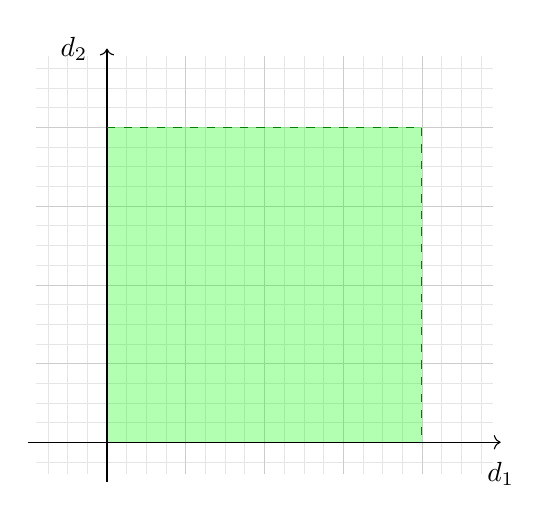
\begin{tikzpicture}
	\coordinate (axis) at (0,0);
	\node at (0,5) [label={180:$d_2$}] {};
	\node at (5,0) [label={-90:$d_1$}] {};
	\draw [step=0.25,draw=black!10!white,very thin] (-0.9,-0.4) grid (4.9,4.9);
	\draw [step=1,draw=black!20!white,very thin] (-0.9,-0.4) grid (4.9,4.9);
	\fill [fill=green,opacity=0.3] (0,0) -- (0,4) -- (4,4) -- (4,0) -- cycle;
	\draw [->] (axis) ++(0,-0.5) -- (0,5);
	\draw [->] (axis) ++(-1,0) -- (5,0);
	\draw [dashed,color={green!50!black}] (axis) (0,4) -- (4,4) -- (4,0);
\end{tikzpicture}

	\caption{Admissible domain and dimming value selection.}
\end{figure}

\section{Arduino data fomat}

{\centering \textit{Provisory section so that Daniel can start the web-server}}

Each Arduino sends data at every sample time so that the server can store the necessary information. 

A message is designed to be a fixed-size word, with the least number of bits possible.
Currently, the message has 20 bytes, as seen in this segment from \texttt{comms.h}:
%\todo[inline]{Minted com xelatex exibe as tabs como \texttt{^^I}. E os underscores, se não fizer escape dão erros com o Tikz.}
\begin{minted}[firstnumber = 20]{c}
typedef struct msg{
    MsgCode code; // 1 byte
    uint8_t address; // 1 byte
    uint8_t aux1; // 1 byte
    uint8_t aux2; // 1 byte
    float value[4]; // 4 x 4 = 16 bytes

}message_t; //size fixed to 20 bytes
\end{minted}

\ccode{code} is an unsigned integer (\ccode{uint8_t}) which represents what the data format is.
Some values for this are used in the callibration procedure, but the value for sample time data forwarding is, for now, 5.
A way of knowing this every time is having the same \ccode{enum} in the server as in the Arduino \texttt{comms} module:
\begin{minted}[firstnumber = 9]{c}
enum MsgCode : uint8_t{

    calibration_request,
    data,
    cont,
    acknowledge,
    consensus_data,
    sampling_time_data,

};
\end{minted}

The rest of the data is:
\begin{table}[ht]
	\centering
	\begin{tabular}[h]{l|l}\toprule
		\ccode{address} & Arduino's I$2$C address. \\
		\ccode{aux1}    & 1st MSB: Desk occupancy state ($1$ for occupied, $0$ for free). \\
		                & next 7 bits, led duty cycle, unsigned integer from $0$ to $100$. \\
		\ccode{aux2}    & Illuminance lower bound (presumably $40$ or $80$), in LUX. \\
		\ccode{value[0]}& Measured illuminance, in LUX. \\
		\ccode{value[1]}& Local background illuminance, in LUX. \\
		\ccode{value[2]}& Instantaneous control illuminance reference, in LUX. \\
		\ccode{value[3]}& Instantaneous power consumption, units to be defined. \\
		\bottomrule
	\end{tabular}
\end{table}

Note, to extract the duty cycle and occupancy state, you can do:
\begin{minted}[linenos=false,frame=none]{c}
  unsigned duty_cycle = aux1 & (0x7F); // This is a bit-wise and with 0111111
  bool state = aux1 & (0x80); // This is a bit-wise and with 10000000 
\end{minted}

From what I see, this is everything we need to send the server, and it should be able to compute the necessary variables. The following table should summarize my thoughts:
\begin{table}[h]
	\centering
	\begin{tabularx}{\linewidth}{l|X}
		Quantity & How to determine (\ccheckmark{} means it is sent every sample time) \\
		Illuminance & \ccheckmark{} \\
		duty cycle  & \ccheckmark{} \\
		occupancy state & \ccheckmark{} \\
		lower bound & \ccheckmark{} \\
		Control reference & \ccheckmark{} \\
		Background illuminance & \ccheckmark{} \\
		Instantaneous power consumption & \ccheckmark{} \\
		Total power consumption & Sum of instantaneous power consumption for all nodes. \\
		Time since last restart & listen to a specific message code (to be defined) and keep the timestamp. \\
		Node energy spent since last restart & integrate node's instantaneous power consumption, sample time is fixed and known. \\
		Total energy since last restart & Sum both nodes's energy spent. \\
		Node confort error since last restart & At each sample time we have the lower bound and the illuminance, do the math. \\
		Total confort error since last restart & Sum both nodes' confort error. \\
		Node flicker since last restart & See project description, all that is needed is the illuminance from the last 3 samples. \\
		Total flicker since last restart & Sum both nodes' flicker.
	\end{tabularx}
\end{table}

I might have missed something, we'll see.

\section{Schematics and Charts}

\begin{figure}
    \centering
    \begin{tikzpicture}
            \begin{axis}
                [width = \linewidth, height = 0.5\linewidth,
                xmin = 0, xmax = 5,
                ymin = 70, ymax = 160,
                xlabel = {Time ($\si{\micro\second}$)},
                ylabel = {Illuminance ($\si{\lux}$)},
                grid = both,
                legend cell align=left,
                legend style={at={(0.5,-0.2)},anchor=north},
                %legend pos = outer north east,
                cycle list = {mark=none},]
            \addplot +[thick,red] table [col sep = comma, x index = 0, y index = 1] {feedback.csv};
            \addplot +[thick,blue] table [col sep = comma, x index = 0, y index = 1] {feedforward.csv};
            \addplot +[thick,green] table [col sep = comma, x index = 0, y index = 1] {feedforward_feedback.csv};
            \addplot +[darkgray,dashed] coordinates {(-2,80) (6,80)};
            \addplot +[darkgray,dashed] coordinates {(-2,150) (6,150)};
            \legend{Pure feedback,Pure feed-forward,Combined,$80$,$150$};
        \end{axis}
    \end{tikzpicture}
    \caption{All those feedback plots in one fine place.}
    \label{fig:feedback}
\end{figure}

\end{comment}

\end{document}
